%$$$$$$$$$$$$$$$$$$$$$$$$$$$$$$$$$$$$$$$$$$$$$$$$$$$$$$$$$$$$$$$$$$$$$$$$$$$$$$$$$$$
%----------------------------------------------------------------------Introducci�n-
\section{Introducci�n}
%$$$$$$$$$$$$$$$$$$$$$$$$$$$$$$$$$$$$$$$$$$$$$$$$$$$$$$$$$$$$$$$$$$$$$$$$$$$$$$$$$$$

% \subsection[Intro]{Definici�n de Tecnolog�a}
% 
% \begin{frame}
%   \frametitle{Tecnolog�a: Definici�n}
%    \begin{center} 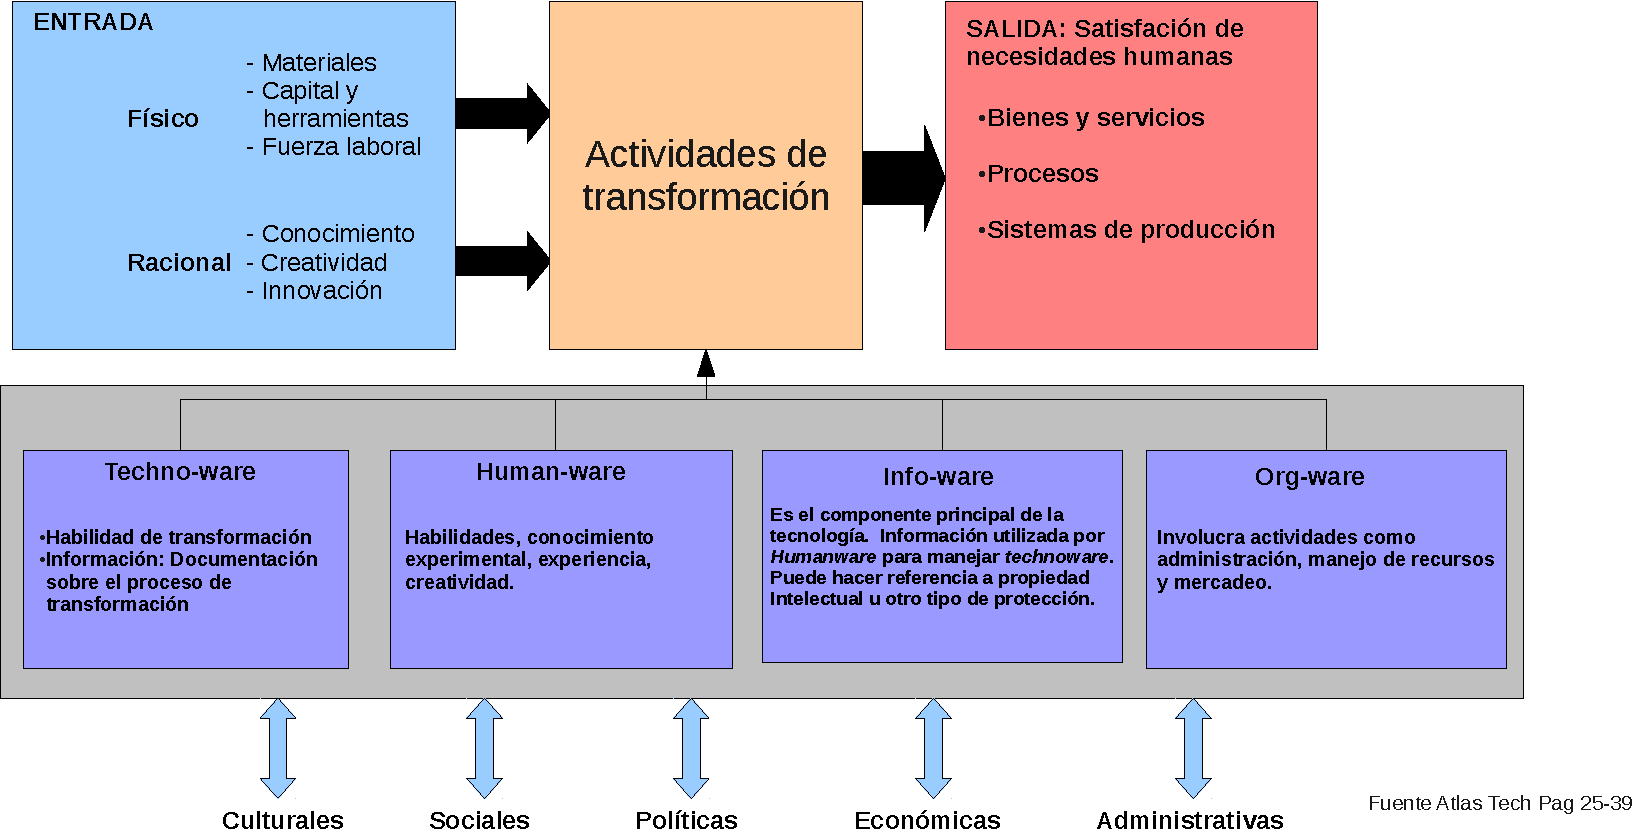
\includegraphics[scale=.45]{../images/technology_definition_slides.pdf}   \end{center}
% \end{frame}

\subsection[Intro]{Transferencia Tecnol�gica}
\begin{frame}
  \frametitle{Transferencia Tecnol�gica}
 
  \begin{alertblock}{}
    \begin{itemize}
     \item<1-> Odedra \cite{Mo94}: \textbf{La transferencia tecnol�gica se considera exitosa cuando los receptores de la tecnolog�a \textcolor{DarkGreen}{asimilan} estos conceptos para \textcolor{DarkGreen}{suplir sus necesidades locales} generando productos novedosos}.
     \item<2-> Jolly \cite{Jol77}: \textbf{El conocimiento es lo que queda al final de un proceso \textcolor{DarkGreen}{documentado y difundido} de forma apropiada. Para que la transferencia tecnol�gica sea exitosa es necesario transferir los componentes de la tecnolog�a}.
    \end{itemize}
  \end{alertblock}

\end{frame}

\subsection{Canales de Transferencia}
\begin{frame}
  \frametitle{Canales para la TT}
   \begin{center} 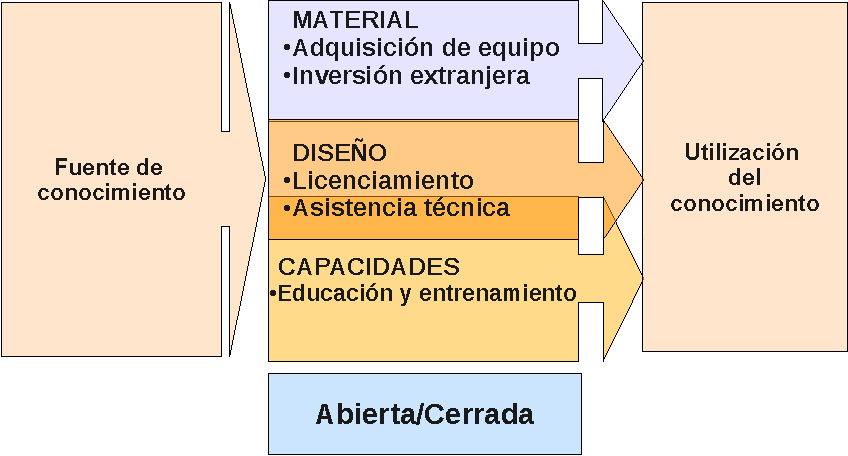
\includegraphics[scale=.6]{../images/TT_canales.pdf}   \end{center}
\end{frame}

\input TT_methodology                  


\section{Rob�tica en la Educaci�n}
\begin{frame}
  \frametitle{Rob�tica en la Educaci�n}

  \begin{block}{}
    La utilizaci�n de la rob�tica en la educaci�n b�sica y media ha venido en aumento, y su uso adecuado permite el desarrollo de habilidades asociadas al constructivismo y al aprendizaje significativo.
  \end{block}
\end{frame}

\begin{frame}
  \frametitle{Utilizaci�n de la rob�tica en la educaci�n}

  \begin{block}{}
    \begin{itemize}
     \item Como objeto de aprendizaje: Enfocado a aspectos relacionados con el robot como construcci�n, programaci�n e inteligencia artificial y la rob�tica.
     \item Como herramienta de aprendizaje: Visto como proyecto interdisciplinario que involucra ciencias, matem�ticas, tecnolog�as de la informaci�n y comunicaciones.
    \end{itemize}
  \end{block}
\end{frame}

\begin{frame}
  \frametitle{Aprender dise�ando}
  \begin{center} 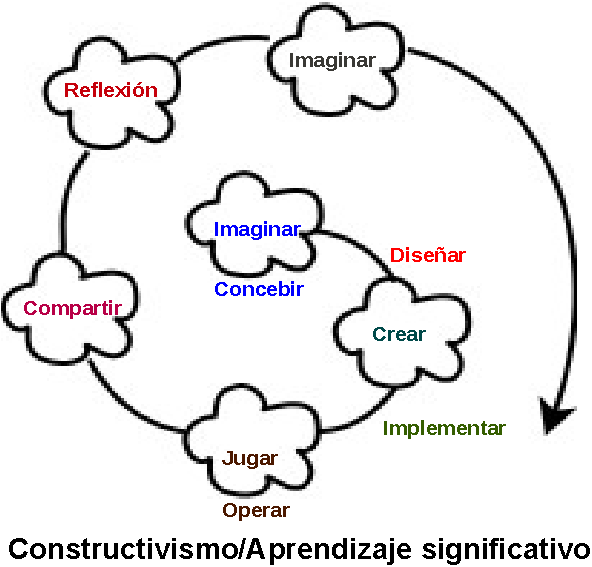
\includegraphics[scale=.7]{../images/siebot2} \end{center}
\end{frame}




